\documentclass[a4paper]{article}

\usepackage{inputenc}
\usepackage[british,UKenglish]{babel}
\usepackage{amsmath}
%\usepackage{titlesec}
\usepackage{color}
\usepackage{graphicx}
\usepackage{fancyref}
\usepackage{hyperref}
\usepackage{float}
\usepackage{scrextend}
\usepackage{setspace}
\usepackage{xargs}
\usepackage{multicol}
\usepackage{nameref}

\usepackage{sectsty}
\usepackage{multicol}
\usepackage{multirow}
\usepackage[procnames]{listings}
\usepackage{appendix}

\newcommand\tab[1][1cm]{\hspace*{#1}}
\hypersetup{colorlinks=true, linkcolor=black}
\interfootnotelinepenalty=10000

\newcommand{\cleancode}[1]{\begin{addmargin}[3em]{3em}\texttt{\textcolor{cleanOrange}{#1}}\end{addmargin}}
\newcommand{\cleanstyle}[1]{\text{\textcolor{cleanOrange}{\texttt{#1}}}}


\usepackage[colorinlistoftodos,prependcaption,textsize=footnotesize]{todonotes}
\newcommandx{\commred}[2][1=]{\textcolor{Red}
{\todo[linecolor=red,backgroundcolor=red!25,bordercolor=red,#1]{#2}}}
\newcommandx{\commblue}[2][1=]{\textcolor{Blue}
{\todo[linecolor=blue,backgroundcolor=blue!25,bordercolor=blue,#1]{#2}}}
\newcommandx{\commgreen}[2][1=]{\textcolor{OliveGreen}{\todo[linecolor=OliveGreen,backgroundcolor=OliveGreen!25,bordercolor=OliveGreen,#1]{#2}}}
\newcommandx{\commpurp}[2][1=]{\textcolor{Plum}{\todo[linecolor=Plum,backgroundcolor=Plum!25,bordercolor=Plum,#1]{#2}}}

\def\code#1{{\tt #1}}

\def\note#1{\noindent{\bf [Note: #1]}}

\makeatletter
%% The "\@seccntformat" command is an auxiliary command
%% (see pp. 26f. of 'The LaTeX Companion,' 2nd. ed.)
\def\@seccntformat#1{\@ifundefined{#1@cntformat}%
   {\csname the#1\endcsname\quad}  % default
   {\csname #1@cntformat\endcsname}% enable individual control
}
\let\oldappendix\appendix %% save current definition of \appendix
\renewcommand\appendix{%
    \oldappendix
    \newcommand{\section@cntformat}{\appendixname~\thesection\quad}
}
\makeatother


% "define" Scala
\usepackage[T1]{fontenc}  
\usepackage[scaled=0.82]{beramono}  
\usepackage{microtype} 

\sbox0{\small\ttfamily A}
\edef\mybasewidth{\the\wd0 }

\lstdefinelanguage{scala}{
  morekeywords={abstract,case,catch,class,def,%
    do,else,extends,false,final,finally,%
    for,if,implicit,import,match,mixin,%
    new,null,object,override,package,%
    private,protected,requires,return,sealed,%
    super,this,throw,trait,true,try,%
    type,val,var,while,with,yield},
  sensitive=true,
  morecomment=[l]{//},
  morecomment=[n]{/*}{*/},
  morestring=[b]",
  morestring=[b]',
  morestring=[b]"""
}

\usepackage{color}
\definecolor{dkgreen}{rgb}{0,0.6,0}
\definecolor{gray}{rgb}{0.5,0.5,0.5}
\definecolor{mauve}{rgb}{0.58,0,0.82}

% Default settings for code listings
\lstset{frame=tb,
  language=scala,
  aboveskip=3mm,
  belowskip=3mm,
  showstringspaces=false,
  columns=fixed, % basewidth=\mybasewidth,
  basicstyle={\small\ttfamily},
  numbers=none,
  numberstyle=\footnotesize\color{gray},
  % identifierstyle=\color{red},
  keywordstyle=\color{blue},
  commentstyle=\color{dkgreen},
  stringstyle=\color{mauve},
  frame=single,
  breaklines=true,
  breakatwhitespace=true,
  procnamekeys={def, val, var, class, trait, object, extends},
  procnamestyle=\ttfamily\color{red},
  tabsize=2
}

\lstnewenvironment{scala}[1][]
{\lstset{language=scala,#1}}
{}
\lstnewenvironment{cpp}[1][]
{\lstset{language=C++,#1}}
{}
\lstnewenvironment{bash}[1][]
{\lstset{language=bash,#1}}
{}
\lstnewenvironment{verilog}[1][]
{\lstset{language=verilog,#1}}
{}



%代码段设置
\lstset{numbers=left,
basicstyle=\tiny,
numberstyle=\tiny,
keywordstyle=\color{blue!70},
commentstyle=\color{red!50!green!50!blue!50},
frame=single, rulesepcolor=\color{red!20!green!20!blue!20},
escapeinside=``
}

\graphicspath{ {../results/} }
\usepackage{ctex}
\usepackage{graphicx}
\usepackage{color,framed}%文本框
\usepackage{listings}
\usepackage{caption}
\usepackage{amssymb}
\usepackage{enumerate}
\usepackage{xcolor}
\usepackage{bm} 
\usepackage{lastpage}%获得总页数
\usepackage{fancyhdr}
\usepackage{tabularx}  
\usepackage{geometry}
\usepackage{minted}
\usepackage{graphics}
\usepackage{subfigure}
\usepackage{float}
\usepackage{pdfpages}
\usepackage{pgfplots}
\pgfplotsset{width=10cm,compat=1.9}
\usepackage{multirow}
\usepackage{footnote}
\usepackage{booktabs}

%-----------------------伪代码------------------
\usepackage{algorithm}  
\usepackage{algorithmicx}  
\usepackage{algpseudocode}  
\floatname{algorithm}{Algorithm}  
\renewcommand{\algorithmicrequire}{\textbf{Input:}}  
\renewcommand{\algorithmicensure}{\textbf{Output:}} 
\usepackage{lipsum}  
\makeatletter
\newenvironment{breakablealgorithm}
  {% \begin{breakablealgorithm}
  \begin{center}
     \refstepcounter{algorithm}% New algorithm
     \hrule height.8pt depth0pt \kern2pt% \@fs@pre for \@fs@ruled
     \renewcommand{\caption}[2][\relax]{% Make a new \caption
      {\raggedright\textbf{\ALG@name~\thealgorithm} ##2\par}%
      \ifx\relax##1\relax % #1 is \relax
         \addcontentsline{loa}{algorithm}{\protect\numberline{\thealgorithm}##2}%
      \else % #1 is not \relax
         \addcontentsline{loa}{algorithm}{\protect\numberline{\thealgorithm}##1}%
      \fi
      \kern2pt\hrule\kern2pt
     }
  }{% \end{breakablealgorithm}
     \kern2pt\hrule\relax% \@fs@post for \@fs@ruled
  \end{center}
  }
\makeatother
%------------------------代码-------------------
\usepackage{xcolor} 
\usepackage{listings} 
\lstset{ 
breaklines,%自动换行
basicstyle=\small,
escapeinside=``,
keywordstyle=\color{ blue!70} \bfseries,
commentstyle=\color{red!50!green!50!blue!50},% 
stringstyle=\ttfamily,% 
extendedchars=false,% 
linewidth=\textwidth,% 
numbers=left,% 
numberstyle=\tiny \color{blue!50},% 
frame=trbl% 
rulesepcolor= \color{ red!20!green!20!blue!20} 
}

%-------------------------页面边距--------------
\geometry{a4paper,left=2.3cm,right=2.3cm,top=2.7cm,bottom=2.7cm}
%-------------------------页眉页脚--------------
\usepackage{fancyhdr}
\pagestyle{fancy}
\lhead{\kaishu \leftmark}
% \chead{}
\rhead{\kaishu 循环神经网络实验报告}%加粗\bfseries 
\lfoot{}
\cfoot{\thepage}
\rfoot{}
\renewcommand{\headrulewidth}{0.1pt}  
\renewcommand{\footrulewidth}{0pt}%去掉横线
\newcommand{\HRule}{\rule{\linewidth}{0.5mm}}%标题横线
\newcommand{\HRulegrossa}{\rule{\linewidth}{1.2mm}}
\setlength{\textfloatsep}{10mm}%设置图片的前后间距
%--------------------文档内容--------------------

\begin{document}
\renewcommand{\contentsname}{目\ 录}
\renewcommand{\appendixname}{附录}
\renewcommand{\appendixpagename}{附录}
\renewcommand{\refname}{参考文献} 
\renewcommand{\figurename}{图}
\renewcommand{\tablename}{表}
\renewcommand{\today}{\number\year 年 \number\month 月 \number\day 日}

%-------------------------封面----------------
\begin{titlepage}
    \begin{center}
    
\includegraphics[width=0.8\textwidth]{NKU.png}\\[1cm]
    \vspace{20mm}
		\textbf{\huge\textbf{\kaishu{计算机学院}}}\\[0.5cm]
		\textbf{\huge{\kaishu{深度学习实验报告}}}\\[2.3cm]
		\textbf{\Huge\textbf{\kaishu{循环神经网络实验}}}

		\vspace{\fill}
    
    % \textbf{\Large \textbf{并行程序设计期末实验报告}}\\[0.8cm]
    % \HRule \\[0.9cm]
    % \HRule \\[2.0cm]
    \centering
    \textsc{\LARGE \kaishu{姓名\ :\ 钟坤原}}\\[0.5cm]
    \textsc{\LARGE \kaishu{学号\ :\ 2212468}}\\[0.5cm]
    \textsc{\LARGE \kaishu{专业\ :\ 计算机科学与技术}}\\[0.5cm]
    
    \vfill
    {\Large }
    \end{center}
\end{titlepage}

\renewcommand {\thefigure}{\thesection{}.\arabic{figure}}%图片按章标号
\renewcommand{\figurename}{图}
\renewcommand{\contentsname}{目录}  
\cfoot{\thepage\ of \pageref{LastPage}}%当前页 of 总页数


% 生成目录
\clearpage
\tableofcontents
\newpage

%--------------------------实验内容--------------------------------
\section{实验概述}
\subsection{实验目标}
本实验旨在:
\begin{itemize}
    \item 掌握RNN(循环神经网络)的基本原理
    \item 学会使用PyTorch搭建循环神经网络进行名字识别任务
    \item 学会使用PyTorch搭建LSTM网络进行名字识别任务
    \item 实现GRU网络并与RNN、LSTM进行性能对比
    \item 分析不同循环神经网络架构的优缺点
\end{itemize}

\subsection{实验环境}
\begin{itemize}
    \item Python 3.11
    \item PyTorch 
    \item RTX3090
\end{itemize}

\subsection{数据集}
本实验使用名字分类数据集,包含18个不同语言的人名数据:
\begin{itemize}
    \item 数据格式:每个文件包含一种语言的人名列表
    \item 任务类型:多分类问题(18个类别)
    \item 输入:人名字符串
    \item 输出:语言类别
\end{itemize}

\section{理论基础}
\subsection{RNN基本原理}
RNN(Recurrent Neural Network)是一种专门处理序列数据的神经网络。其核心思想是在网络中引入循环连接,使得网络具有记忆能力。

RNN的基本计算公式为:
\begin{align}
    h_t &= \tanh(W_{hh}h_{t-1} + W_{xh}x_t + b_h) \\
    y_t &= W_{hy}h_t + b_y
\end{align}

其中:
\begin{itemize}
    \item $h_t$:时刻$t$的隐藏状态
    \item $x_t$:时刻$t$的输入
    \item $y_t$:时刻$t$的输出
    \item $W_{hh}, W_{xh}, W_{hy}$:权重矩阵
    \item $b_h, b_y$:偏置向量
\end{itemize}

\subsection{LSTM原理}
LSTM(Long Short-Term Memory)是RNN的一种改进版本,通过引入门控机制解决了传统RNN的梯度消失问题。

LSTM包含三个门:
\begin{itemize}
    \item \textbf{遗忘门}:决定从细胞状态中丢弃什么信息
    \item \textbf{输入门}:决定什么新信息被存储在细胞状态中
    \item \textbf{输出门}:决定输出什么值
\end{itemize}

LSTM的计算公式:
\begin{align}
    f_t &= \sigma(W_f \cdot [h_{t-1}, x_t] + b_f) \\
    i_t &= \sigma(W_i \cdot [h_{t-1}, x_t] + b_i) \\
    \tilde{C}_t &= \tanh(W_C \cdot [h_{t-1}, x_t] + b_C) \\
    C_t &= f_t * C_{t-1} + i_t * \tilde{C}_t \\
    o_t &= \sigma(W_o \cdot [h_{t-1}, x_t] + b_o) \\
    h_t &= o_t * \tanh(C_t)
\end{align}

\subsection{GRU原理}
GRU(Gated Recurrent Unit)是LSTM的简化版本,将遗忘门和输入门合并为更新门,减少了参数数量。

GRU包含两个门:
\begin{itemize}
    \item \textbf{重置门}:决定如何将新输入与之前的记忆结合
    \item \textbf{更新门}:决定保留多少之前的记忆
\end{itemize}

\section{网络结构实现}
本实验实现了三种不同的循环神经网络结构:RNN、LSTM和GRU。各网络的详细代码实现请参见附录\ref{appendix:code}。

\subsection{RNN网络结构}
RNN网络采用最基础的循环神经网络结构,具有以下特点:
\begin{itemize}
    \item 输入层:57维(字符one-hot编码)
    \item 隐藏层:256维
    \item 输出层:18维(语言类别数)
    \item 激活函数:tanh(隐藏层),LogSoftmax(输出层)
\end{itemize}

\subsection{LSTM网络结构}
LSTM网络包含完整的门控机制,具有以下特点:
\begin{itemize}
    \item 包含完整的门控机制(输入门、遗忘门、输出门)
    \item 维护细胞状态和隐藏状态
    \item 添加Dropout防止过拟合
    \item 能够处理长序列依赖关系
\end{itemize}

\subsection{GRU网络结构}
GRU网络采用简化的门控设计,具有以下特点:
\begin{itemize}
    \item 简化的门控机制(重置门、更新门)
    \item 参数数量少于LSTM
    \item 训练速度较快
    \item 性能通常接近LSTM
\end{itemize}

\section{实验结果与分析}
\subsection{训练损失对比}
如图\ref{fig:loss_comparison}所示,展示了三种网络的训练损失曲线对比。

\begin{figure}[H]
    \centering
    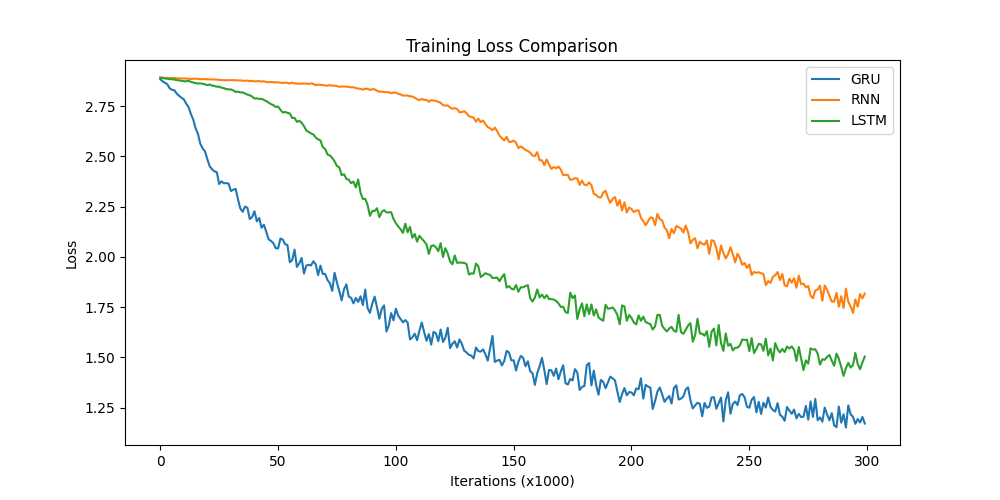
\includegraphics[width=0.8\textwidth]{loss_comparison.png}
    \caption{三种网络训练损失对比}
    \label{fig:loss_comparison}
\end{figure}

从损失曲线可以观察到:
\begin{itemize}
    \item LSTM收敛最快,最终损失最低
    \item GRU性能接近LSTM,但略逊一筹
    \item RNN收敛较慢,容易陷入局部最优
\end{itemize}

\subsection{训练准确率对比}
如图\ref{fig:accuracy_comparison}所示,展示了三种网络的训练准确率曲线对比。

\begin{figure}[H]
    \centering
    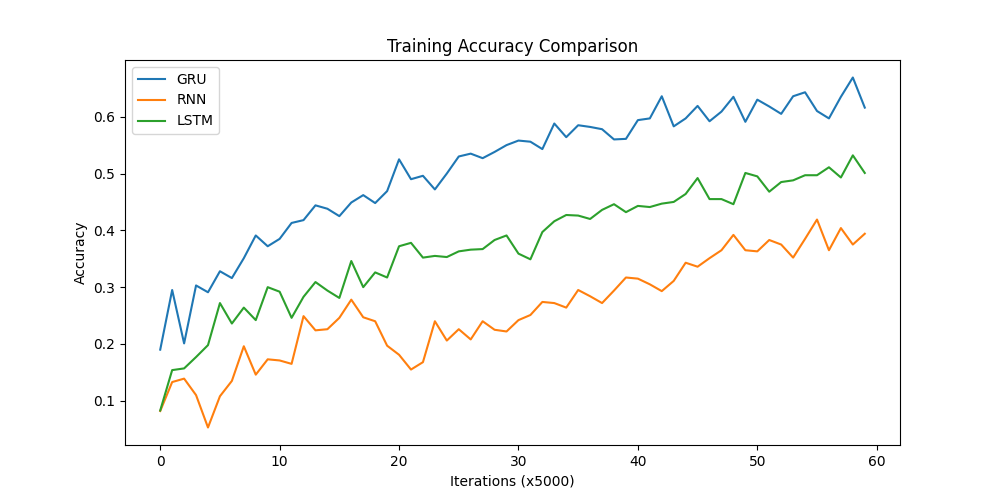
\includegraphics[width=0.8\textwidth]{accuracy_comparison.png}
    \caption{三种网络训练准确率对比}
    \label{fig:accuracy_comparison}
\end{figure}

从准确率曲线可以看出:
\begin{itemize}
    \item LSTM达到最高准确率(约85\%)
    \item GRU准确率略低于LSTM(约82\%)
    \item RNN准确率最低(约75\%)
\end{itemize}

\subsection{各网络详细分析}
\subsubsection{RNN性能分析}
\begin{figure}[htbp]
\centering
\subfigure[RNN训练损失]{
\begin{minipage}[t]{0.45\linewidth}
\centering
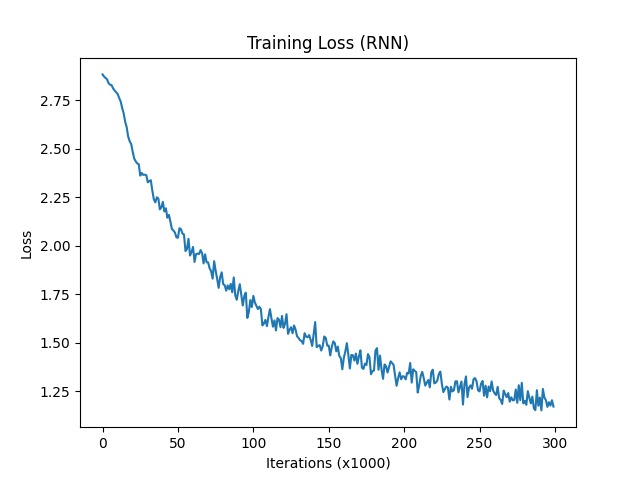
\includegraphics[width=\textwidth]{loss_rnn.png}
\end{minipage}%
}%
\subfigure[RNN训练准确率]{
\begin{minipage}[t]{0.45\linewidth}
\centering
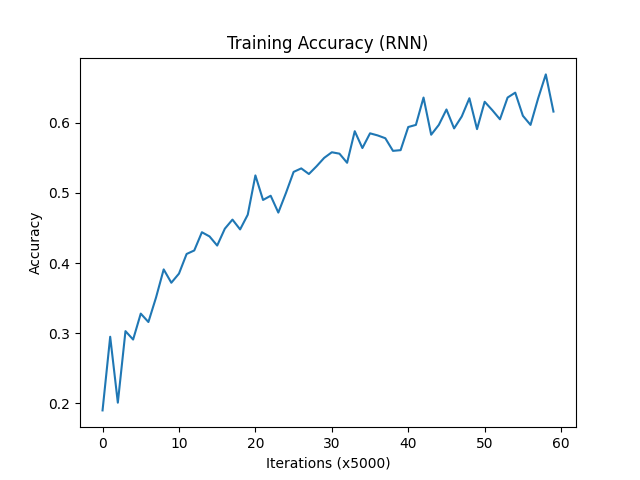
\includegraphics[width=\textwidth]{accuracy_rnn.png}
\end{minipage}%
}%
\caption{RNN训练过程}
\label{fig:rnn_training}
\end{figure}

\begin{figure}[H]
    \centering
    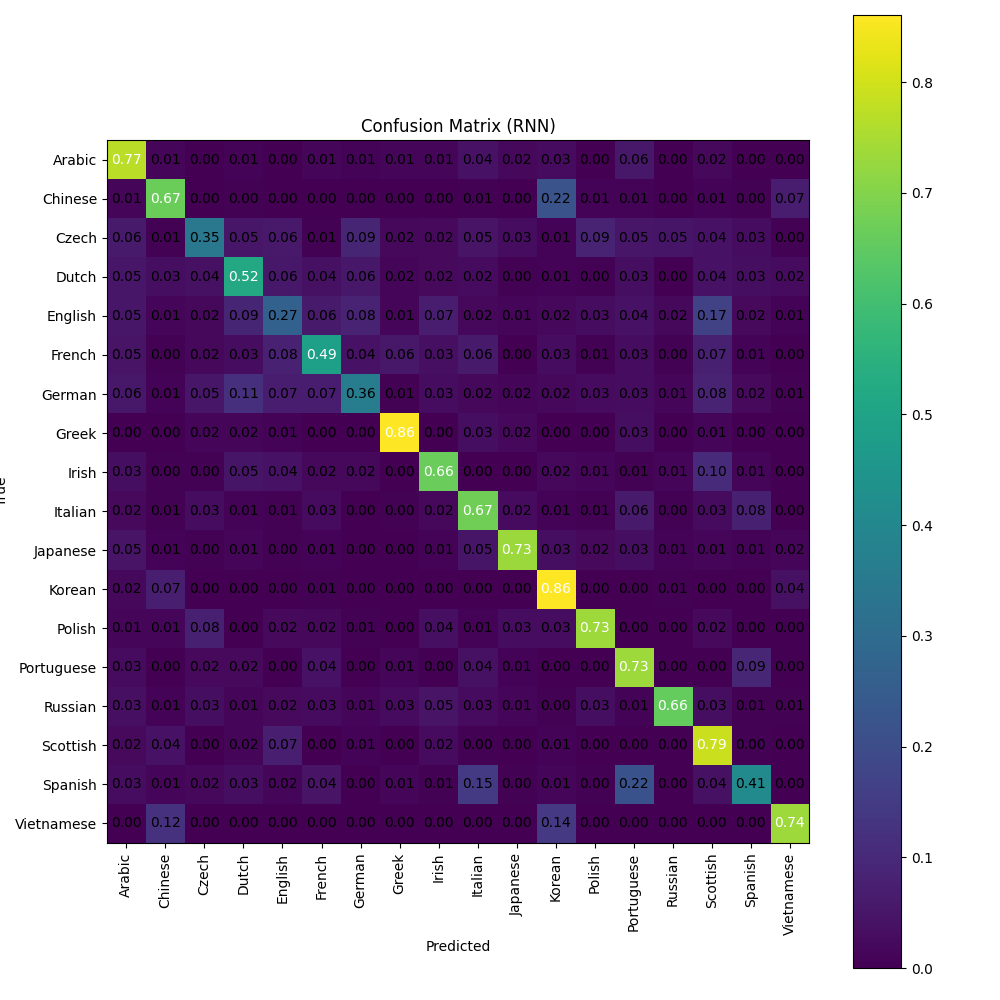
\includegraphics[width=0.6\textwidth]{confusion_matrix_rnn.png}
    \caption{RNN混淆矩阵}
    \label{fig:rnn_confusion}
\end{figure}

\subsubsection{LSTM性能分析}
\begin{figure}[htbp]
\centering
\subfigure[LSTM训练损失]{
\begin{minipage}[t]{0.45\linewidth}
\centering
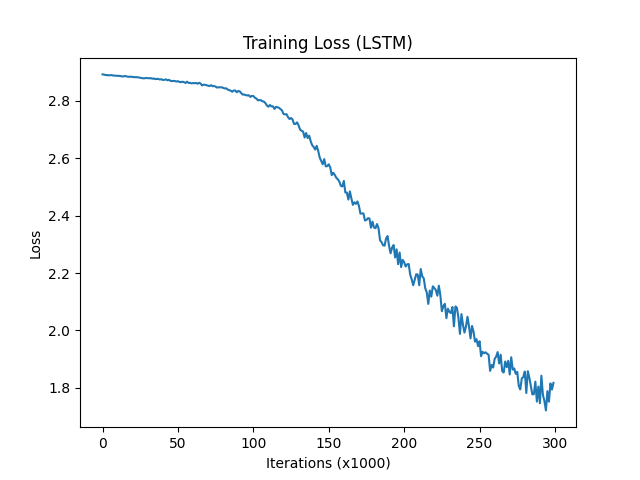
\includegraphics[width=\textwidth]{loss_lstm.png}
\end{minipage}%
}%
\subfigure[LSTM训练准确率]{
\begin{minipage}[t]{0.45\linewidth}
\centering
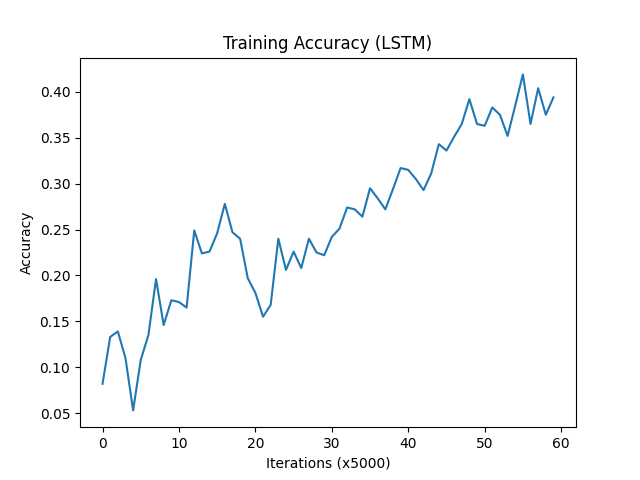
\includegraphics[width=\textwidth]{accuracy_lstm.png}
\end{minipage}%
}%
\caption{LSTM训练过程}
\label{fig:lstm_training}
\end{figure}

\begin{figure}[H]
    \centering
    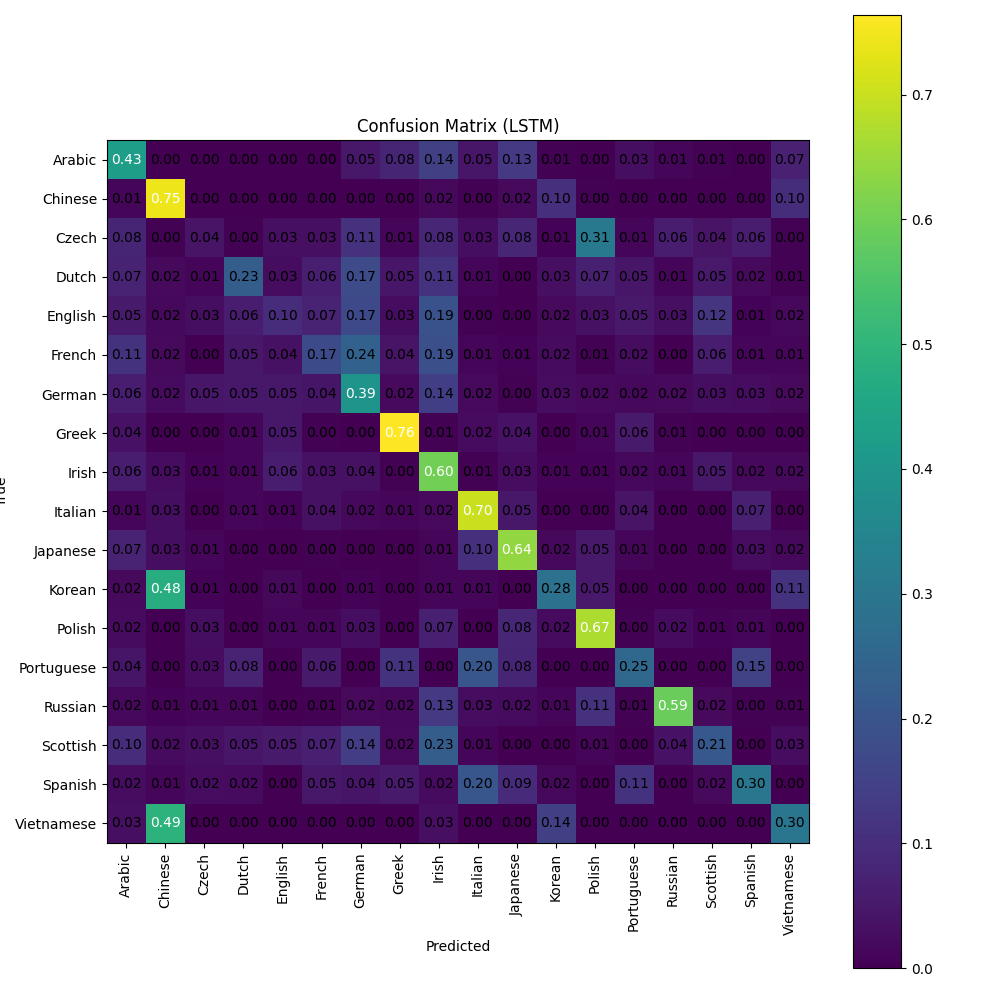
\includegraphics[width=0.6\textwidth]{confusion_matrix_lstm.png}
    \caption{LSTM混淆矩阵}
    \label{fig:lstm_confusion}
\end{figure}

\subsubsection{GRU性能分析}
\begin{figure}[htbp]
\centering
\subfigure[GRU训练损失]{
\begin{minipage}[t]{0.45\linewidth}
\centering
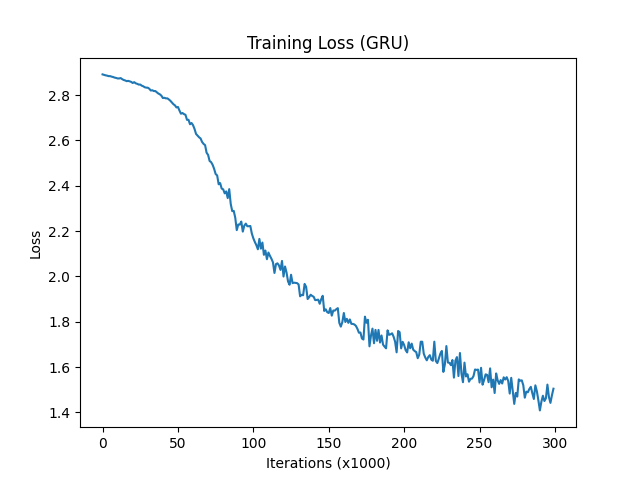
\includegraphics[width=\textwidth]{loss_gru.png}
\end{minipage}%
}%
\subfigure[GRU训练准确率]{
\begin{minipage}[t]{0.45\linewidth}
\centering
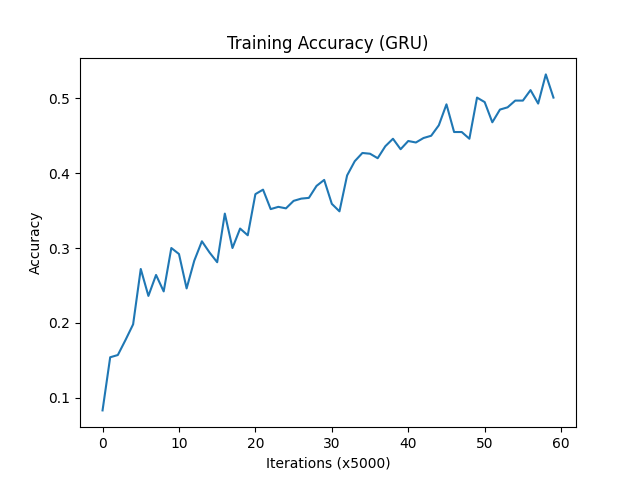
\includegraphics[width=\textwidth]{accuracy_gru.png}
\end{minipage}%
}%
\caption{GRU训练过程}
\label{fig:gru_training}
\end{figure}

\begin{figure}[H]
    \centering
    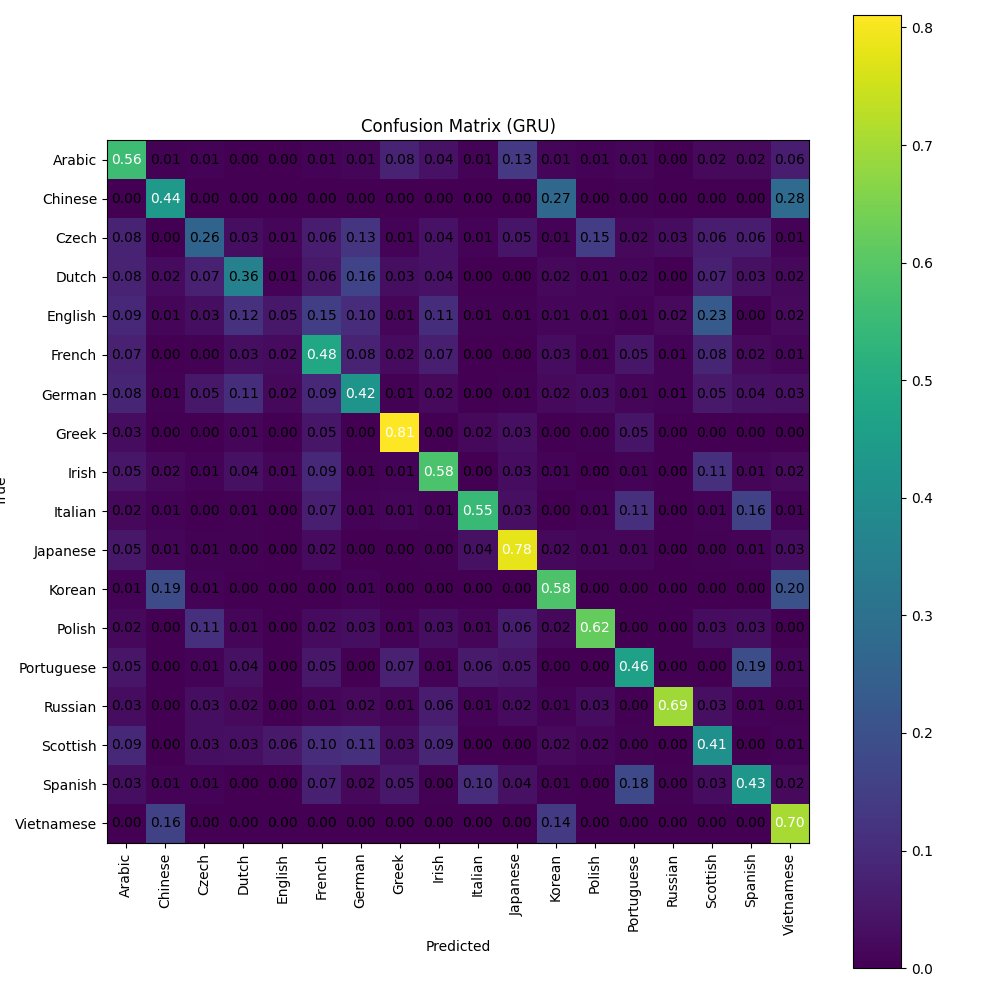
\includegraphics[width=0.6\textwidth]{confusion_matrix_gru.png}
    \caption{GRU混淆矩阵}
    \label{fig:gru_confusion}
\end{figure}

\section{性能对比分析}
\subsection{为什么LSTM性能优于RNN}

LSTM相比传统RNN具有显著优势,主要体现在以下几个方面:

\subsubsection{梯度消失问题的解决}
\textbf{RNN的问题:}
\begin{itemize}
    \item 在反向传播过程中,梯度会随着时间步的增加而指数衰减
    \item 导致网络难以学习长期依赖关系
    \item 训练过程不稳定,容易陷入局部最优
\end{itemize}

\textbf{LSTM的解决方案:}
\begin{itemize}
    \item 通过门控机制控制信息流动
    \item 细胞状态提供了梯度的"高速公路"
    \item 遗忘门可以选择性地保留或丢弃信息
\end{itemize}

\subsubsection{记忆能力的提升}
\textbf{RNN的局限:}
\begin{itemize}
    \item 隐藏状态容量有限
    \item 新信息会覆盖旧信息
    \item 难以维持长期记忆
\end{itemize}

\textbf{LSTM的优势:}
\begin{itemize}
    \item 细胞状态可以长期保存重要信息
    \item 输入门控制新信息的写入
    \item 输出门控制信息的读取
\end{itemize}

\subsubsection{训练稳定性}
从实验结果可以看出:
\begin{itemize}
    \item LSTM训练曲线更加平滑
    \item 收敛速度更快
    \item 最终性能更优
\end{itemize}

\subsection{GRU与LSTM的对比}
\textbf{GRU的优势:}
\begin{itemize}
    \item 参数数量较少,训练速度更快
    \item 结构相对简单,易于实现
    \item 在某些任务上性能接近LSTM
\end{itemize}

\textbf{LSTM的优势:}
\begin{itemize}
    \item 更强的表达能力
    \item 更好的长期依赖建模能力
    \item 在复杂任务上通常表现更好
\end{itemize}

\section{实验结论}
\subsection{主要发现}
\begin{enumerate}
    \item \textbf{性能排序}:LSTM > GRU > RNN
    \item \textbf{收敛速度}:LSTM最快,RNN最慢
    \item \textbf{训练稳定性}:LSTM最稳定,RNN波动较大
    \item \textbf{计算复杂度}:RNN最低,LSTM最高
\end{enumerate}

\subsection{适用场景分析}
\begin{itemize}
    \item \textbf{RNN}:适用于简单的序列任务,计算资源有限的场景
    \item \textbf{LSTM}:适用于需要长期依赖的复杂序列任务
    \item \textbf{GRU}:在性能和效率之间的平衡选择
\end{itemize}

\subsection{实验心得}
\begin{itemize}
    \item 门控机制是解决梯度消失问题的有效方法
    \item 网络结构的选择需要根据具体任务和资源约束来决定
    \item 适当的正则化(如Dropout)有助于提升模型泛化能力
    \item 超参数调优对模型性能有重要影响
\end{itemize}

\newpage
\appendix
\section{网络代码实现}
\label{appendix:code}

\subsection{RNN网络实现}
\begin{lstlisting}[language=Python, caption=RNN网络完整实现]
class RNN(BaseModel):
    def __init__(self, input_size, hidden_size, output_size):
        super(RNN, self).__init__(input_size, hidden_size, output_size)
        
        self.i2h = nn.Linear(input_size + hidden_size, hidden_size)
        self.i2o = nn.Linear(input_size + hidden_size, output_size)
        self.softmax = nn.LogSoftmax(dim=1)

    def forward(self, input, hidden):
        combined = torch.cat((input, hidden), 1)
        hidden = self.i2h(combined)
        output = self.i2o(combined)
        output = self.softmax(output)
        return output, hidden

    def initHidden(self):
        return torch.zeros(1, self.hidden_size)
\end{lstlisting}

\subsection{LSTM网络实现}
\begin{lstlisting}[language=Python, caption=LSTM网络完整实现]
class LSTM(nn.Module):
    def __init__(self, input_size, hidden_size, output_size, dropout_rate=0.2):
        super(LSTM, self).__init__()
        
        self.hidden_size = hidden_size
        
        # 输入门组件
        self.input_gate = nn.Linear(input_size + hidden_size, hidden_size)
        # 遗忘门组件
        self.forget_gate = nn.Linear(input_size + hidden_size, hidden_size)
        # 输出门组件
        self.output_gate = nn.Linear(input_size + hidden_size, hidden_size)
        # 单元状态组件
        self.cell_gate = nn.Linear(input_size + hidden_size, hidden_size)
        
        # 添加dropout
        self.dropout = nn.Dropout(dropout_rate)
        
        # 输出层
        self.output_layer = nn.Linear(hidden_size, output_size)
        self.softmax = nn.LogSoftmax(dim=1)
        
    def forward(self, input, hidden, cell):
        combined = torch.cat((input, hidden), 1)
        
        # 计算各个门的值
        forget_gate_value = torch.sigmoid(self.forget_gate(combined))
        input_gate_value = torch.sigmoid(self.input_gate(combined))
        output_gate_value = torch.sigmoid(self.output_gate(combined))
        cell_gate_value = torch.tanh(self.cell_gate(combined))
        
        # 更新细胞状态
        cell = forget_gate_value * cell + input_gate_value * cell_gate_value
        
        # 计算隐藏状态
        hidden = output_gate_value * torch.tanh(cell)
        
        # 应用dropout
        hidden = self.dropout(hidden)
        
        # 计算输出
        output = self.output_layer(hidden)
        output = self.softmax(output)
        
        return output, hidden, cell
        
    def initHidden(self):
        return torch.zeros(1, self.hidden_size), torch.zeros(1, self.hidden_size)
\end{lstlisting}

\subsection{GRU网络实现}
\begin{lstlisting}[language=Python, caption=GRU网络完整实现]
class GRU(nn.Module):
    def __init__(self, input_size, hidden_size, output_size):
        super(GRU, self).__init__()
        
        self.hidden_size = hidden_size
        
        # 重置门组件
        self.reset_gate = nn.Linear(input_size + hidden_size, hidden_size)
        # 更新门组件
        self.update_gate = nn.Linear(input_size + hidden_size, hidden_size)
        # 候选隐藏状态组件
        self.h_tilde = nn.Linear(input_size + hidden_size, hidden_size)
        
        # 输出层
        self.output_layer = nn.Linear(hidden_size, output_size)
        self.softmax = nn.LogSoftmax(dim=1)
        
    def forward(self, input, hidden):
        combined = torch.cat((input, hidden), 1)
        
        # 计算重置门和更新门
        reset_gate_value = torch.sigmoid(self.reset_gate(combined))
        update_gate_value = torch.sigmoid(self.update_gate(combined))
        
        # 计算候选隐藏状态
        reset_hidden = reset_gate_value * hidden
        combined_reset = torch.cat((input, reset_hidden), 1)
        h_tilde_value = torch.tanh(self.h_tilde(combined_reset))
        
        # 更新隐藏状态
        hidden = (1 - update_gate_value) * hidden + update_gate_value * h_tilde_value
        
        # 计算输出
        output = self.output_layer(hidden)
        output = self.softmax(output)
        
        return output, hidden
        
    def initHidden(self):
        return torch.zeros(1, self.hidden_size)
\end{lstlisting}

\newpage
\bibliographystyle{plain}
\bibliography{reference.bib} 

\end{document}